
\documentclass{aa}  

\usepackage{graphicx}
%%%%%%%%%%%%%%%%%%%%%%%%%%%%%%%%%%%%%%%%
\usepackage{txfonts}
\usepackage{multirow}
%%%%%%%%%%%%%%%%%%%%%%%%%%%%%%%%%%%%%%%%
%\usepackage[options]{hyperref}
% To add links in your PDF file, use the package "hyperref"
% with options according to your LaTeX or PDFLaTeX drivers.
%
  % methods heading (mandatory)
  % {Methods}
%   Aims. The HIFI pipeline was designed to provide robust conversion from raw telemetry into calibrated data throughout all phases of
%the HIFI missions. Pre-launch laboratory testing was supported as were routine mission operations.
%Methods. A modular software design allowed components to be easily added, removed, amended and/or extended as the understanding
%of the HIFI data developed during and after mission operations.
%Results. The HIFI pipeline processed data from all HIFI observing modes within the Herschel automated processing environment as
%well as within an interactive environment. The same software can be used by the general astronomical community to reprocess any
%standard HIFI observation. The pipeline also recorded the consistency of processing results and provided automated quality reports.
%Many pipeline modules were in use since the HIFI pre-launch instrument level testing.
%Conclusions. Processing in steps facilitated data analysis to discover and address instrument artefacts and uncertainties. The availabil-
%ity of the same pipeline components from pre-launch throughout the mission made for well-understood, tested, and stable processing.
%A smooth transition from one phase to the next significantly enhanced processing reliability and robustness.
%}
  % results heading (mandatory)
\begin{document} 


   \title{Data processing pipelines and the data center for the X-ray spectrometer / imager STIX onboard Solar Orbiter}

   \subtitle{}

   \author{Hualin Xiao
          \inst{1}
          \and 
          Shane Maloney 
          \inst{2}
          \and 
          Ewan Dickson \inst{1,4}
          \and 
          S\"am Krucker\inst{1}
          \and Andrea Francesco Battaglia\inst{3}
            \and László Etesi \inst{1}
         % \and Ryan Daniel \inst{1}
         % \and Lastufka Erica \inst{1}
          \and Other STIX team members
         }

   \institute{University of Applied Sciences and Arts Northwestern Switzerland (FHNW), 5200 Windisch, Switzerland \\
              \email{hualin.xiao@fhnw.ch}
         \and
          Astrophysics Research Group, School of Physics, Trinity College Dublin, Dublin 2, Ireland
          \and
             ETH Z\"urich, R\"amistrasse 101, 8092 Z\"urich, Switzerland
         \and University of Graz, Universitätspl. 3, 8010 Graz, Austria
             }

   \date{}

% \abstract{}{}{}{}{} 
% 5 {} token are mandatory
 
  \abstract
  % context heading (optional)
   {} %leave it empty if necessary  
  % {context.}
  % aims heading (mandatory)
   { The Spectrometer/Telescope for Imaging X-rays (STIX) instrument onboard the Solar Orbiter mission launched on February 10, 2020 promises advances in the study of solar flares of various sizes. It is capable of measuring X-ray spectra from 4 to 150 keV with 1 keV resolution binned into 32 energy bins before downlinking. STIX data center is an infrastructure established at FHNW in order to process and archive STIX telemetry data, and to support the operations of the instrument. The automated data processing pipelines turn raw telemetry data into processed information and data products. Processed information and data products are achived at the data center.  STIX data center provides the solar physics community various tools to visualize STIX data products.
   }

   {Results.}
  % conclusions heading (optional), leave it empty if necessary 
   {}

   \keywords{Solar flares --Data Center --
                STIX data products --
                Data processing pipeline
               }

   \maketitle
%
%-------------------------------------------------------------------

\section{Introduction}
Solar Orbiter is a Sun-observing mission of the European Space  Agency that 
addresses the interaction between the Sun and the heliosphere.
It was launched on Feb. 10, 2020 for a nominal mission duration of seven years and a planned 
extension of
three years. It carries ten sets of instruments for comprehensive
remote-sensing and in-situ measurements. 
Solar Orbiter  will perform detailed measurements of the Sun as close as 0.28 AU and for the first time look at its uncharted polar regions (\cite{SolarOrbiter2020}).  
Its goal is to  address the center question of heliophysics  "How does the Sun create and control the heliosphere?".  It is designed to identify the origins and causes of the solar wind, the heliospheric magnetic field, the solar energetic particles, the transient interplanetary disturbances, and the Sun's magnetic field.
This consists of the study of energetic solar phenomena like flares,  solar transients,  the solar wind accelerating mechanisms, and the solar dynamo principle.  


The Spectrometer Telescope for Imaging X-rays (STIX) is one of the instruments onboard Solar Orbiter.  
It measures X-rays from 4 to 150 keV and takes X-ray images with a few arcsec angular resolution by using an indirect imaging technique based on the Moiré effect. 
STIX instrument consists of 32 collimators with
grids and pixelated Cadmium telluride detector units called Caliste-SO.
The main science objective of STIX is to study the extremely hot solar plasma and the high-energy electrons accelerated during solar flares. STIX will address the key science goals of the Solar Orbiter mission by providing information on intensity, 
spectrum, timing, and location of accelerated electrons near the Sun.
For details of the STIX instrumentation, we refer to the instrument paper \cite{StixInstrument}.


During nominal science operations, STIX continuously acquires science data. 
They are processed and compressed into different types of telemetry packets by
before being transmitted to the ground.
Being aware of the complexity of STIX data analysis and 
the need of bringing the data to the solar physics community, a data center has been
developed at FHNW. The data center (SDC) receives, analyzes, archives and distributes STIX data,
 and supports STIX in-flight operations.
It turns raw telemetry data into processed information and produces data products that can be used for scientific analysis.
It also provides various data visualization tools to the solar physics community.
The purpose of this paper is to describe the standard processing pipelines, 
algorithms of automated data processing, data products and tools provided by the STIX data center.
%We will describe here STIX data types,  the flow of data from to the users, the data processing pipelines, the %database, the data products and the tools provided for the solar physics comnunity.
%--------------------------------------------------------------------

This paper is organized as follows: Section \ref{sec:raw-data} briefly introduces STIX raw telemetry types, Data flow and telemetry
We end with a summary in Section \ref{sec:summary}.
\section{STIX raw telemetry data}
\label{sec:raw-data}

STIX continuously observes high-energy events on the Sun at 4 -- 150keV. 
Photons emitted by solar flares are detected with 32 subcollimators 
(a 12-pixel-detector behind a front and rear grid). While passing through the front and rear grids, 
the flares generate a modulation pattern over the 12 pixels of each detector. 
The pattern can then be used to reconstruct images and to do spectroscopy. 
Other data products include lightcurves, flare information, spectra, and background information.
The nominal telemetry budget of STIX is 50 bps.
STIX is far from earth, not all data can be downloaded from the spacecraft. We have low latency data.
For bulk science data have to be requested.
STIX continuously collects energy deposition information from 32 detector units, the aspect system,
and engineering sensors in the nominal observation mode.
The collected data are first processed by the FPGA and the onboard flight software
After the prompt processing, low latency telemetry data are directed to the
storage in the spacecraft whearas high time resolution pixel data are written to STIX onboard archive memory for
later processings.
STIX transmits data to the spacecraft in the form of binary packets.
STIX raw telemetry data can be classified into four
categories: housekeeping data, diagnostic data, quick-look data and science data.

In the next sections, we briefly introduce the main raw telemetry data types.
For details about STIX raw telemetry data, we refer to STIX instrument paper \cite{StixInstrument}.

\subsection{Housekeeping data}
 %\item  Housekeeping data.
 %STIX generates two different houskeeping data packets.
STIX housekeeping data (HK) contain engineering data that measure temperatures, voltages, currents, status of switches,
averaged signal readouts from the four aspect photodiodes, detector trigger counts, and  flags indicating
status bits of the onboard software and the archive memoery.
The data is used to monitor instrument status, and the instrument pointing.
%All the parameters are reported in the same type packet at a fixed 64 sec cadence.
HK data are generated as long as STIX is powered on.
During nominal operations, a housekeeping packet is generated every 64 seconds, which results in a daily raw telemetry of  143 kiB.
All STIX sensors and the IDPU will produce housekeeping data that will be received on ground with the highest priority
for monitoring instrument status and health.

\subsection{Quick-look data}
STIX has only one operational mode in which Low Latency data is produced, and that is  NOMINAL mode, which is the regular science mode.
STIX generates four different types of quick-look (QL) data:
\begin{itemize}
                                                                                                                                                               \item Quick-look light curves, which are time series of counts
of all pixels in 30 detectors (excluding background detector and the coarse flare locator)
accumulated every 4 sec time resolution in five broad energy ranges (two thermal, two nonthermal
and one intermediate). Quick-look light curves are generated when STIX is in nominal observation mode.
STIX light curves are a time series of detector counts in different energy bands (units will be counts/second/cm$^2$). There are five configurable energy bands (for example: 4-7keV, 7-11keV, 11-16keV, 16-40keV, and 40-150keV), with a default integration time of 4 seconds. A lightcurve data point corresponds to the total counts integrated over all selected detectors and pixels for the given energy band. The data are temperature corrected on-board, and undergo minor corrections for detector and pixels,
and nominal grid transmission (25 percent) on the ground. As lower energies are highly impacted by the presence of the attenuator, they will also need to be corrected. The data will not be corrected for background, live time or detector efficiency. The FITS file is in accordance with [LLFITSICD] but will also comply with  in order to be usable with existing high-energy solar data file routines.

The light curve data are structured as an array of five count values COUNTS (for the five energy bands) per time, where time is a relative time $RELATIVE_TIME$ since $OBT_START$ that is time bin centered (i.e. with an integration time of 4s, $RELATIVE_TIME$ will 2-6-10…, as opposed to 0-4-8…). It is possible that that $RELATIVE_TIME$ “jumps”, e.g. when the attenuator is moving in and the affected time bin becomes undetermined and is left out. Additionally, there is an energy channel reference CHANNEL, with indices into the energy axis in the second extension. Given below is an IDL-based structure notation.

\item Background monitor light curves. Background monitor light curves are similar to the Quick-look light curves but only
counts recorded by the background detector pixels are included, and the integration time is 8 seconds.
\item Variance data are   onboard computed variance of 40 successive detector-summed count rates
based on 0.1 sec integration.
\item Quick-look spectra, which are energy snapshots of energy spectra (32 science energy bins) for
each of the 32 detectors with 32 sec exposure time.
STIX takes a snapshot of energy spectra every 1024
seconds in the nominal observation mode.
\item Calibration spectra. Calibration spectra are accumulated for events from the weak onboard $^{133}$Ba radioactive sources over long periods (typically 24 hours) when the solar count rate is small compared to background.
The identification of such quiet periods is done autonomously, based on the presence of a
TC-specified time gap between successive photons.  The relevant portions of these
spectra are included in the quick-look low-latency data.
\end{itemize}
\subsection{Diagnostic and event data}
When a failure is detected directly by STIX, the instrument’s response includes sending a
“dedicated” telemetry event report with appropriate diagnostic information included.

\subsection{Bulk science data}

Bulk science data are different combinations of summing and compression of the basic pixel data stored in STIX onboard archive memory, which can be used for spectrocopy and imaging.
To cope with the limited available telemetry, they are not automatically included in the telemetry.
Onboard formation of the science data is invoked by data request telecommands.
Each science request can select subsets of energies, pixels and detectors.
Six different science data can be generated:
\begin{itemize}
 \item Level-0 X-ray data is the least processed data and contains uncompressed counts for the selected energies, pixels and detectors;
\item Level-1 is essentially the same as Level-0 but the counts are compressed onboard before being sent to the ground;
\item Level-2 data are further compressed counts from the L1 pixel data, in which are summed down to 4 before compression.
\item Level-3 data are visibilities, which further reduces the data by combine the the 4 summed pixel counts into a complex visibility which is also compressed.
\item Level-4 data are detector summed spectrograms;
\item High-time resolution aspect data.
\end{itemize}
\begin{table}[h]
\centering
\caption{STIX raw telemetry data coverage, data rate and typical reception delay at SDC.  }
\resizebox{0.5\textwidth}{!}{
\begin{tabular}{lllll}
\hline
Category &  Coverage &Daily data volume & Reception Delay  \\ \hline
Housekeeping           & continous &   143 kiB  & hours to days \\ \hline
Quicklook     & continous         & $\sim$ 358 kiB  & hours to days   \\ \hline

Science     & ground-selected only &  $\sim$ MiB to $\sim$ 10 MiB &  2 to 12 weeks   \\ \hline
Calibration  & quiet sun periods  & 100 kiB  & $\sim$ 1 day \\ \hline
\end{tabular}
}
\label{tb:raw_types}
\end{table}

Housekeeping data, quick-look data and calibration data are directed to the
common low latency data stored in SSMM in the spacecraft.
The coverage, data rate and latency of
different types of STIX raw telemetry data are
summarized in Table \ref{tb:raw_types}.

%https://issues.cosmos.esa.int/solarorbiterwiki/display/SOSP/SOC+Archive+Plan?preview=%2F11734040%2F21759347%2FSOL-SGS-PL-0009-SOARPL-2.0.pdf

\section{Data reception}

During nominal science operations,
Low latency data are down-linked in the very next ground station pass regardless of orbital geometry, 
whereas science data are only downlinked when the bandwidth permits.
The downloaded instrument telemetry data are first processed by ESA's ground segment
software at the Solar Orbiter mission control center. Then they
are distributed to instrument teams by the ESA EGOS Data
Dissemination System (EDDS) (\cite{EDDS}) according instrument teams' preset conditions.


Telemetry data received by STIX data center from EDDS  are in binary format, 
and  they have the same structure as the data generated by STIX instrument.
The delay of low-latency data ranges from a few hours to a few days, depending on whether there
are antenna passes, whearas science data may arrive several weeks after being generated onboard.


In addition to the telemetry data, STIX data center also receives SPICE kernel files (\cite{spice})  from the science operations center.
The SPICE kernels contain information of spacecraft ephemeris and clocking calibration factors required for time conversions.


\section{Data processing pipelines}
\subsubsection{Raw data parsing}

\begin{figure*}
    \centering
    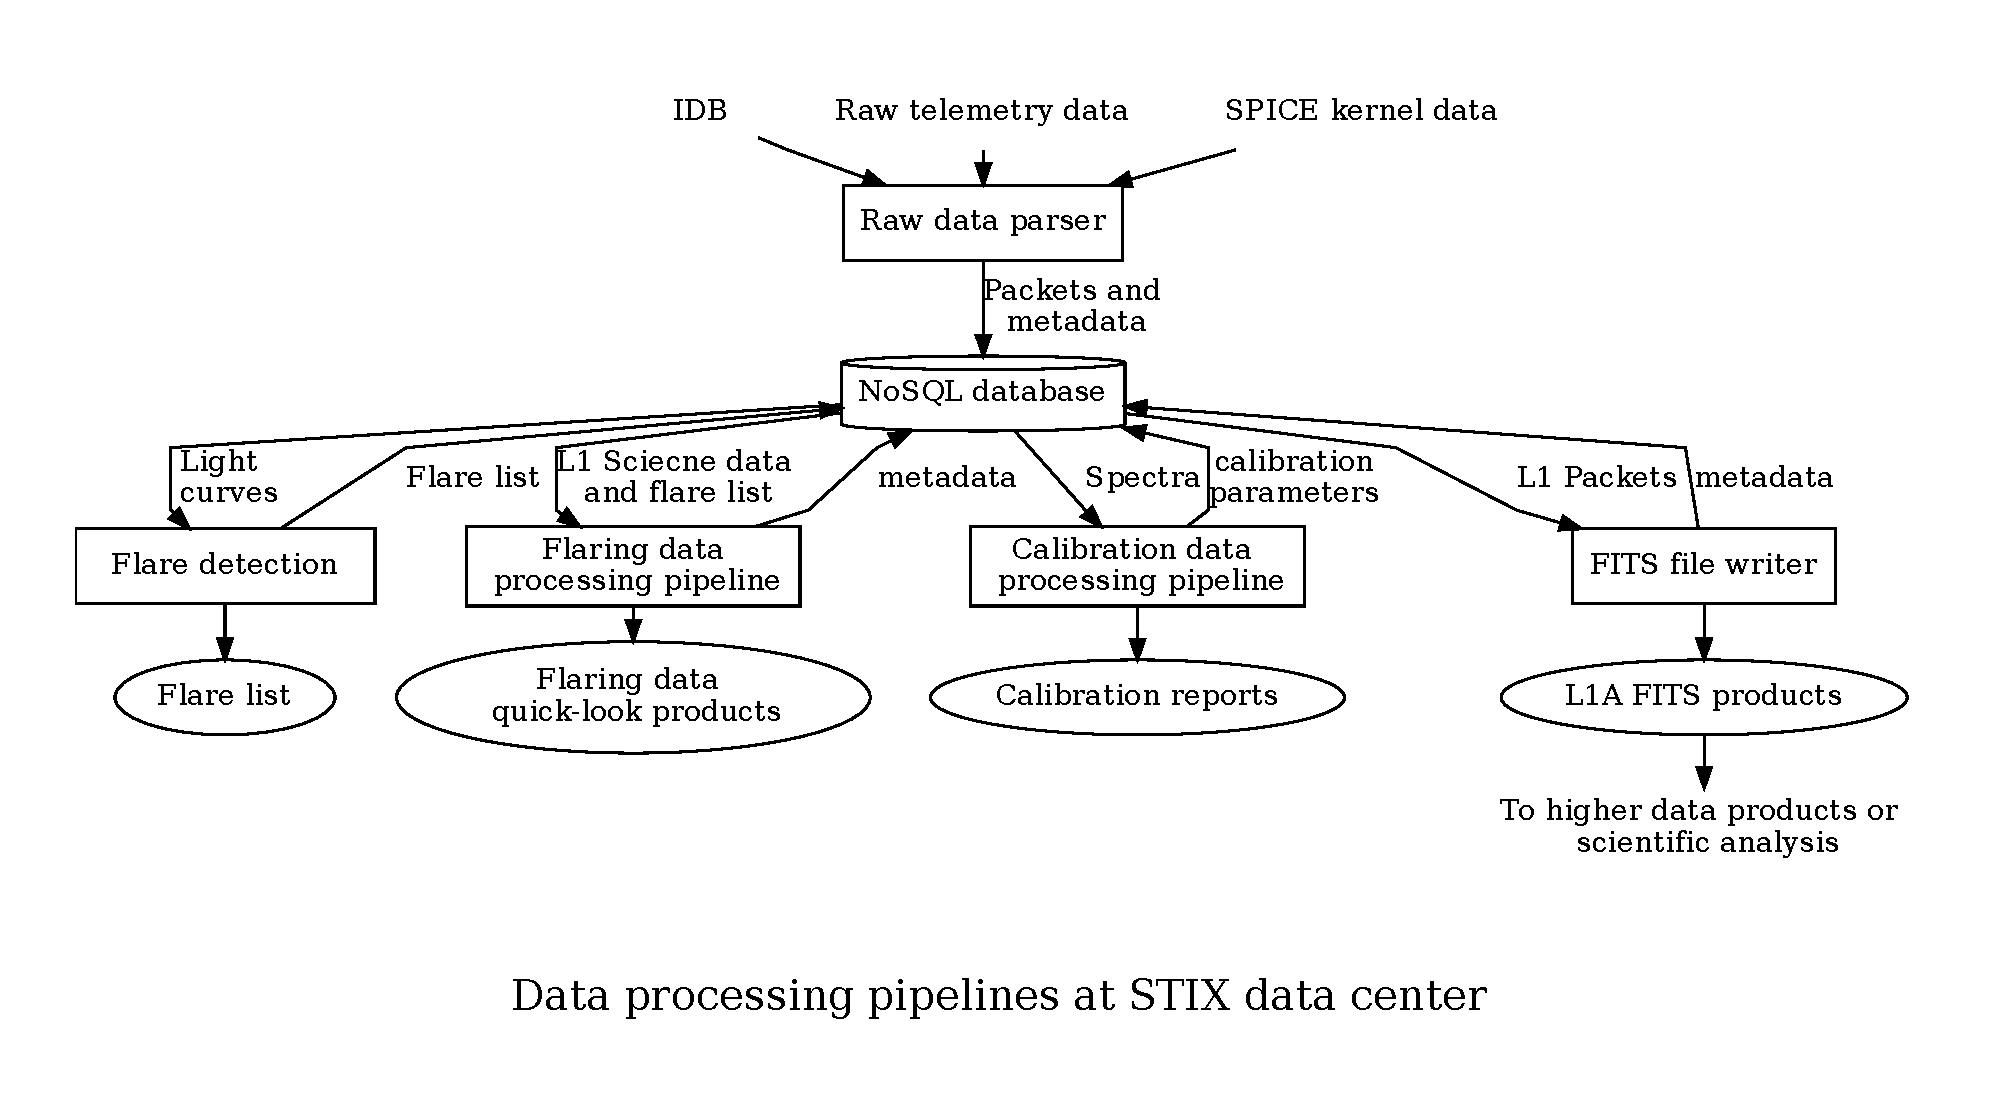
\includegraphics[width=0.9\textwidth]{figures/pipelines.pdf}
    \caption{Data processing pipelines at STIX data center.}
    \label{fig:main_pipelines}
\end{figure*}

%https://v000658.fhnw.ch/index.php/apps/files/?dir=/Stix/GSW/documents&fileid=1206862
New telemetry data arrived at STIX data center are processed by STIX data parser immediately. 
The parser is able to decode all types of STIX binary telecommands and telemetry packets.   
Decoding of raw binary data is based on the mission interface database (MIB), which 
contains  information on packet parameters such as  names, descriptions, lengths,
data types. Decoded packets contain raw values of parameters. For spacecraft clock times,
they are further converted to UTC times using 
SPICE kernel tools (\cite{spice}), compressed integers are  
decompressed by using a LUT table and  housekeeping raw values are converted to 
human-readable values using calibration factors or look-up tables stored in the MIB. 
Packets after above processing steps  are called level-1 packets, they
 are stored in tree structures.  
 They are written to a high-performance NoSQL database, no matter what types they are. 
The NoSQL database is schemaless, making it ideal to store data with complex structures but small sizes. 

During the data parsing,  the parser also extract metadata  such as,  data arrival 
times, data acquisition  time ranges,  calibration run numbers,  raw data 
filenames and SPICE kernel versions.  They are also written to the NoSQL but different collections. 
They are needed by the subsequent processing pipelines. 




\subsubsection{FITS file creation}


\section{Filename naming conventions}

\subsection{STIX raw data processing pipeline}

\subsubsection{Background data processing pipeline}
Light curves measured during quiet periods of the sun are used for background estimation. Median values and of counts are computed and considered as the background in the selected time frame. They are stored in a database and used for flare identifications. 

\subsection{Calibration data processing pipeline}
The calibration data processing pipeline is started automatically after the calibration data raw packets
are being parsed and written to the NoSQL database.


As described in Ref. \cite{StixInstrument},  Ba134 radioactive sources with a total activity of about 4000 Bq are placed at the front of each detector. The total activity of the radioactive source is approximately 4000 Ba.
When the radioactive source decays, gamma rays are generated. These gamma rays can form peaks in the energy spectrum of the detector.
As the energies of the peaks are known, and the corresponding relationship between ADC and real energy can be calibrated through the position of the peak in the energy spectrum, that is, the calibration coefficient. The figure below is a typical Ba133 gamma-ray energy spectrum measured by STIX CdTe detector. There are three obvious peaks in the energy spectrum, and they correspond to three energies of 30 keV, 35 keV and 81 keV. There are many ways to determine the position of each peak, you can use the ECC method, or use the Gaussian function to fit the left part of the peak.


ELUT and calibratino factors can be downloaded from STIX data center by using web GUIs or python APIs.
\subsubsection{Calibration analysis production, ELUT}

\section{Data request procedure}

For detected flares,  a script is used to create data requests.
If the background subtracted peak count rate of a flare is greater 150,
both L1 and spectrogram requests are created;  For micro-flares, as only
spectrograms are request normally as the statistics is too
low to reconstruct flare images.  Aspect data requests
and some extra data requests are created for events of interest in the
STIX operations team.
For external users, data request forms can be also submitted using a web tool
at the data center.

An unique ID is assigned to each data request automatically.
The ID naming convention is yyddmmxxxx, in which yyddmm indicate the observation year (without century), month, date,
and the last four digits indicates the serial number of the data request in the day.
IDs are used to track the status of data requests, and reterieve data products from the
STIX data center.
The information of created data requests are stored in the NoSQL database on the same server.
They are converted to instrument operation requests (IORs) after a series of checks.
Requested data will arrive at STIX data center within a time frame of two weeks to three months, depending on
telemetry allocations.


\section{Flare processing pipeline}

\subsubsection{Flare identification}
Quick-look light curves in the energy range 4 to 10 keV are used for solar flare identification.  The flare identification procedure consists of  two steps:
\begin{itemize}
\item Light curve smoothing. In order to filter spikes from electronics and to reduce the amount of variation due to statistics and the onboard integer compression, light curves are smoothed by using the average filtering. The
\item Flare identification. Local maximums are selected from smoothed light curves.  A local maximum is considered as a flare peak if the counts are exceeds 2 standard deviations above the background and the duration above the background is longer than 1 minute.
\end{itemize}

For each of identified solar flares,   the  information such as start time, end time, counts, background subtracted counts is stored in the STIX flare database.   It is used for automatic creation of data requests for on-board archived data.

How to define a flux.

An ID is given to each identified solar flares. 

\subsubsection{Flare ID naming convention}
\subsubsection{Determination of solar flare GOES classes}

\begin{figure}
  \centering
  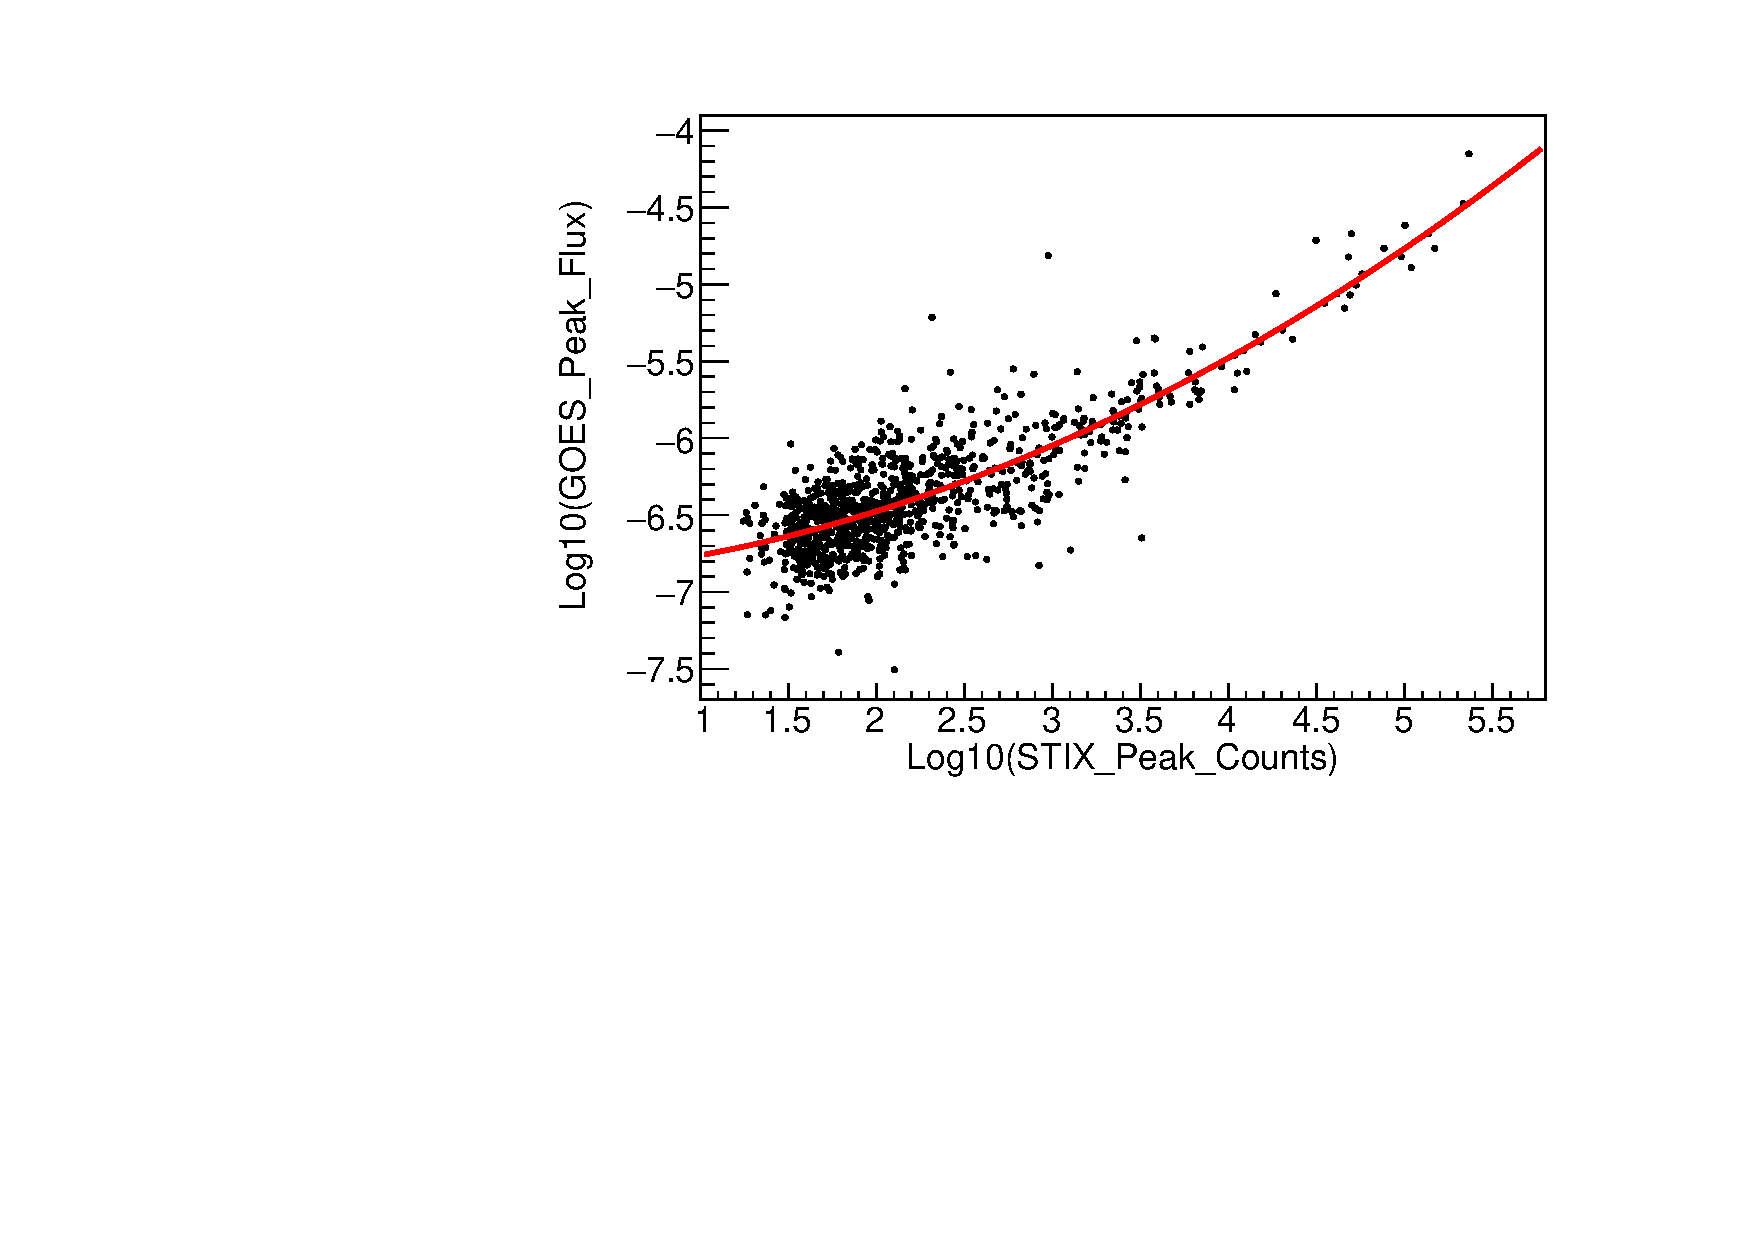
\includegraphics[width=0.8\linewidth]{figures/goes-stix-scatter.pdf}
  \caption{A scatter plot of GOES flux and STIX peak counts in the 4 -- 10 keV quick-look light curve for 989 flares observed by both instruments.
A quadratic function fitted to the log-log data is also shown in the figure. 
STIX counts are background subtracted and 
corrected for flux differences due to the variation of the distance between the Sun and Solar Orbiter. 
The fitted parameters for the quadratic function  are $p_0$=-6.91, $p_1$=0.075 and $p_2$=0.071. 
}
\label{fig:goes-stix}
\end{figure}
For flares that are not observed by GOES. 
A model based on a polynomial fit to the relationship of GOES flux between  STIX counts normalized by the 
squared distance between the Sun and STIX (More details about the model.
Fig. \ref{fig:goes-stix} shows the correlation between GOES flux and STIX peak counts in the 4 -- 10 keV quick-look light curve
for 989 flares observed before Jan. 2022 by both instruments. 
The GOES flux of a solar flare $F$ is estimated using
\begin{equation}
F=10^{p_0+p_1 x+p_2 x^2},
\end{equation}
with
\begin{equation}
 x=\log_{10} {c*r^2}.
\end{equation}
where $p_0$, $p_1$, $p_2$ are the parameters from the curve fit, 
$c$ is STIX background subtracted  counts accumulated in 4 sec and $r$ is 
the distance between the Sun and solar orbiter in units of AU, respectively.
The error of an estimated flux is considered to be the same as the error 
of its nearest data point.

\subsubsection{Flare locations}

\begin{figure*}
  \centering
  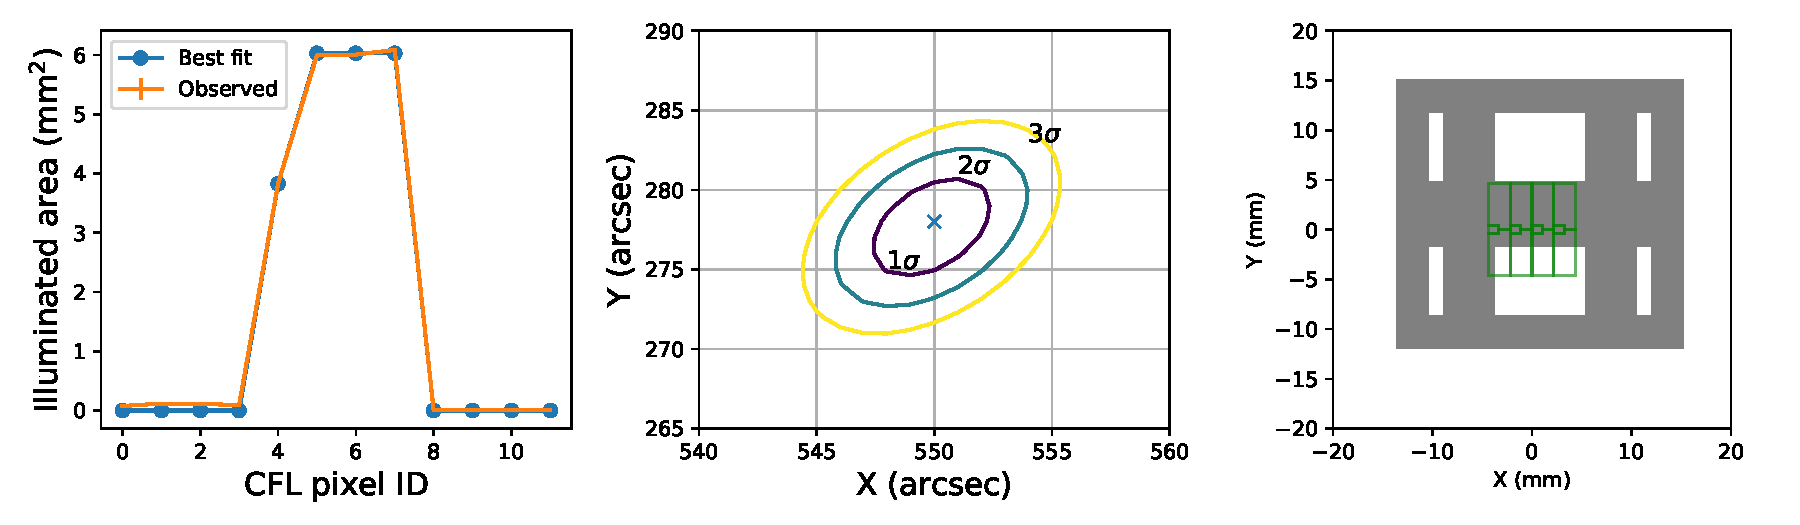
\includegraphics[width=0.95\linewidth]{figures/cflMay07.pdf}
  \caption{Left: area of exposed regions of 12 pixels calculated by combining
  the twelve pixels counts with averages from other detectors, and the best fit.
   Middle: solution of flare location as seen by Solar Orbiter for Flare 202105070034.
   The best fit location is indicated with the symbol X. The 1 $\sigma$, 2 $\sigma$ and 3 $\sigma$ confidence
   regions are also shown. Right: shadow of CFL sub-collimator projected on the twelve CFL pixels.}
  \label{fig:cflpattern}
  %/FHNW/STIX/SolarFlareAnalysis/stix_simulator/cfl
\end{figure*}




\begin{figure*}
  \centering
  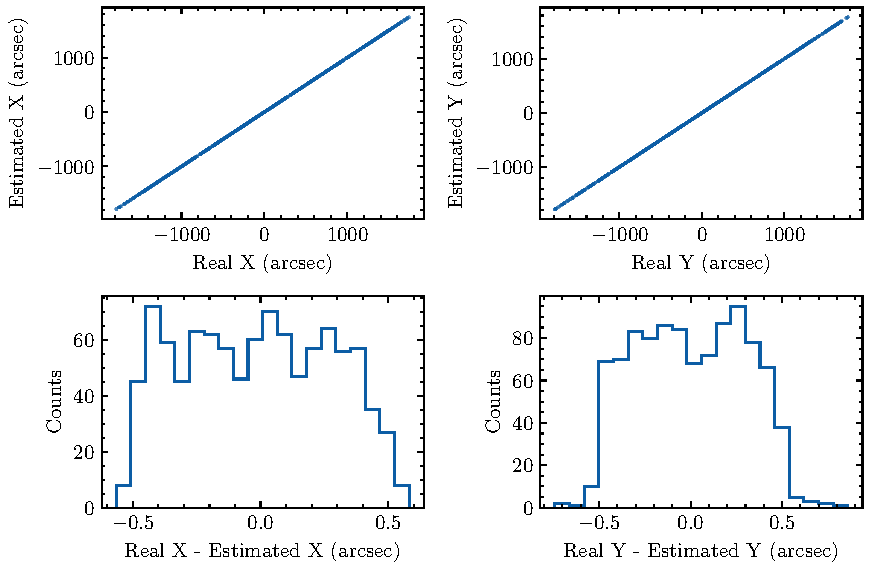
\includegraphics[width=0.7\linewidth]{figures/cflError.pdf}
  \caption{Top: reconstructed coarse flare location solutions against actual locations along the x-axis (left) and y-axis (right). Bottom:
  Differences between the reconstructed and randomly generated locations along
   the x-axis (left) and y-axis (right). The generated sources are assumed to be point-like. Note that statistical
   uncertainties are not considered here. 
    }
  \label{fig:cflerror}
  %/FHNW/STIX/SolarFlareAnalysis/stix_simulator/cfl
\end{figure*}




\subsection{Solar flare list}
\subsection{Flare location database}


A list of products from the flare processing pipeline

* Flare list
* Flare location
*

\subsubsection{Flare location using coarse flare data}
\subsubsection{Flare classification using GOES x-ray flux}

\section{STIX data products}

\subsection{L1 data products}
\begin{itemize}
    \item Raw data.
    \item L1 data.
    \item L2 data
    
\end{itemize}

The latest level 1 FITS IO from Shane has been integrated into the data processing pipeline on pub023 server.

I have recreated fits products for all old telemetry data with the upgraded SW.

The L1 fits files  created by this pipeline have a different data level:  L1A ('A' here means  prerelease/alpha version).

The idea behind L1A data sets is to allow for quicker access to STIX data in the fits format instead of grabbing  data from plots or using JSON requests,

for operations,  debugging  etc.

The L1A data sets can be generated within a few minutes after the arrival of a new raw telemetry file.

The differences between L1A and L1 available in Shane's ftp include:

1.  Two different L1A data files may have duplicated data

2.  L1A data sets are still created for incomplete packets  (L1 checks for data completeness)

3.  SPICE kernel data for telemetry files always arrives  after one or two days later.
    So  there may be a sub-second difference between the UTC time in fits files (same to times on web pages)

   and the real time.

    Shane's formal L1 release can avoid this issue if they are produced on a later date.

4. L1A contains housekeeping data

The different data-processing levels for HMI are summarized as follows, with more details available from this source:
• Data at Level 0 are images that have been constructed from the raw telemetry stream.
• Data at Level 1.0 are images that have been converted from Level 0, with processing including bad-pixel removal, flat-fielding,
and quality assessment checks, but otherwise not having undergone any irreversible data alterations.
• Data at Level 1.5 are images of the physical observables (Dopplergrams, magnetograms, and continuum images), which were
constructed from the individual Level 1.0 filtergrams.
• Data at Level 2 have been irrevocably filtered, time-sequence-merged, Fourier-transformed or otherwise changed from Level 1.5
data in a way that is irreversible. Level 2 products include intermediate products for later production of mission science data
products, such as helioseismic inferences of solar subsurface flows


The Level0 archive contains TM which has been parsed or decommuated into readable structures but no additional external information is include:

times are not converted to UTC
no calibration or conversions applied
for STIX we need to decide if we decompress / combine X-ray L0 the count/trigger data at this stage or in the next level L1

copy manual,
tree like, 
json formats
name, raw value, eng value, children
look-up table, to know description

estimate mongodb benchmark
Mongodb benchmark,
key value, index, performance


\subsection{Auxilary data}



\begin{table}
\centering
\caption{Level 1 data products}
\begin{tabular}{llll}
Category & Type   &  Naming convention  & Remarks   \\ \hline
 Housekeeping & hk\_mini  &  & Houskeeping in BOOT mode   \\
 & hk\_maxi  &  & houskeeping data in NOMINAL   \\
 Quick-look &  light curves &  & Quicklook lightcurves \\
  &  variance &  & variance \\
  &  spectra &  &  \\
  &  background monitor &  &  \\
    &  flare location &  &  \\
 Calibration data &   &  &  \\
\end{tabular}
\end{table}
\section{data request principle}

\section{Database}
\subsection{Raw data packet database } 
\subsection{Configuration database}

\section{Online data visualization tools}
\subsection{Quick-look light curve}
\subsection{Science data quick analysis}
\subsubsection{Calibration data}
\begin{figure}
    \centering
    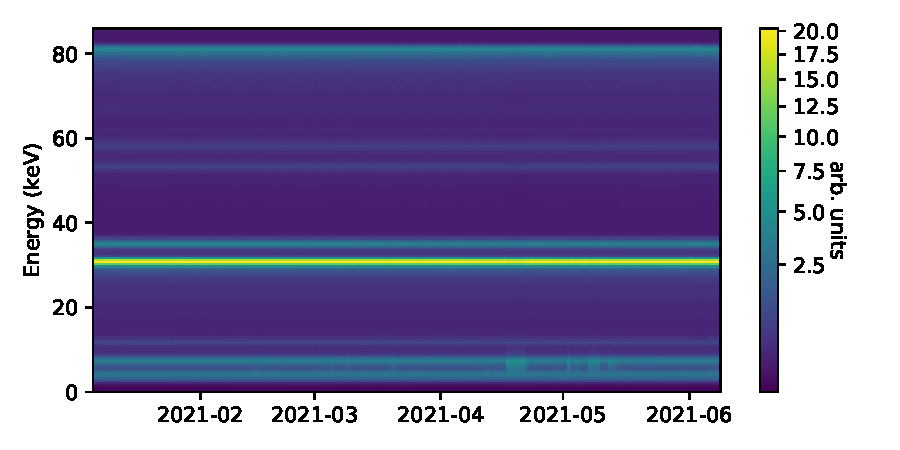
\includegraphics[width=0.8\linewidth]{figures/calibrationSpectrogram.pdf}
    \caption{Caption}
    \label{fig:calibrationSpectrum}
\end{figure}
\begin{figure}
    \centering
    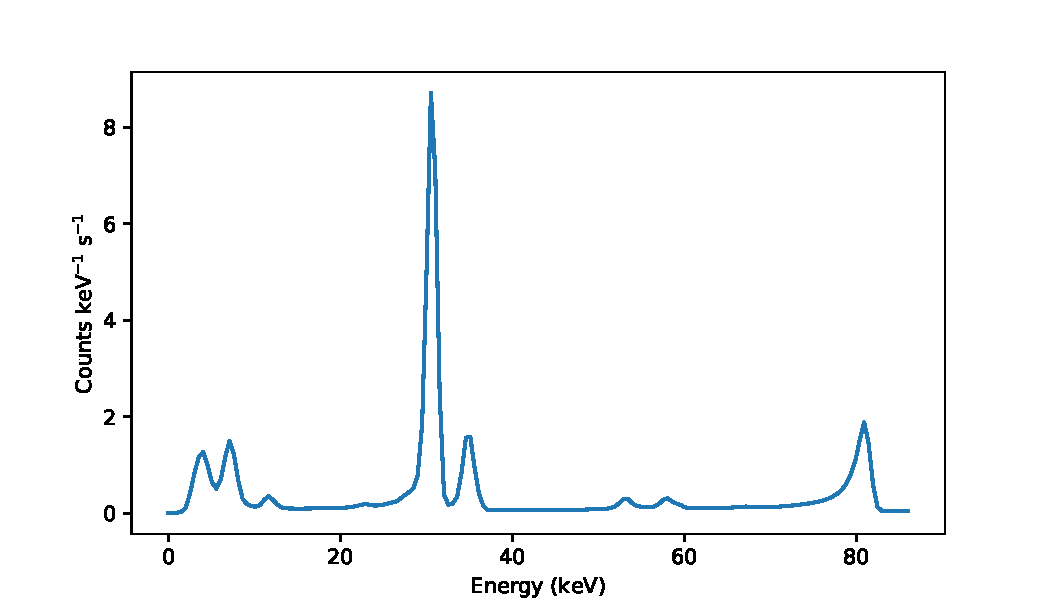
\includegraphics[width=0.8\linewidth]{figures/calibrationSpectrum.pdf}
    \caption{Spectrogram of STIX calibration spectra}
    \label{fig:calibrationSpectrogram}
\end{figure}

calibration data products
https://fermi.gsfc.nasa.gov/ssc/data/access/gbm/
\subsubsection{Solar Orbiter orbit viewer}


When a new data file from the platform is received at the PPDC,
it triggers an autonomous start of the dedicated program that decodes and
interprets its contents. The binary data contain the spacecraft location, attitude, speed, and GPS timestamps with increments every half second. The GPS timestamps are converted into Unix-timestamps, where the leap seconds are also considered. After processing, the platform data are written to the ROOT format files. The data start and stop time, data processing time, input filename and ID of the output file of each processing are recorded in a dedicated database table.
SPICE kernel

Updated once per day.

At the center of the Sun.
It is worth mentioning that has to corrected for.
This can be done by using the web tool provided at the auxiliary data center at

\subsection{Automated data request scheme}
scheme


\section{Data access and APIs}
stixdcpy allows you to query and download data which are available at STIX data center, include
Quick-look light curves
Housekeeping data
Science data
Energy calibration data
Auxilary data
STIX solar flare list


\section{Summary}
\label{sec:summary}



% WARNING
%-------------------------------------------------------------------
% Please note that we have included the references to the file aa.dem in
% order to compile it, but we ask you to:
%
% - use BibTeX with the regular commands:
%   \bibliographystyle{aa} % style aa.bst
%   \bibliography{Yourfile} % your references Yourfile.bib
%
% - join the .bib files when you upload your source files
%-------------------------------------------------------------------

\bibliographystyle{aa}
\bibliography{citations}

\end{document}
